\def\thisdir{science/veryhighz/}


\section{Search for Galaxies at $z>7$ with Narrow-Band Imaging
\label{sec:nbf}}

\noindent
\begin{center}
%% Authors
{\bf Ikuru Iwata$^{1}$, Masayuki Akiyama}\\
$^1$ Subaru Telescope, National Astronomical Observatory of Japan, 650
North Aohoku Place, Hilo, HI 96720, USA
\end{center}
\vspace{0.5cm}

\subsection{Introduction}

Subaru has been one of leading facilities pushing the frontier of
the distant universe. A unique capability of the prime focus camera
(Suprime-Cam) have enabled us to conduct wide-field survey which is
essentially important to find very rare objects such as luminous distant
galaxies. One of the efficient methods to find distant star-forming
galaxies is to detect Ly$\alpha$ emission using narrow-band filter (NBF) 
imaging. A strongly star-forming object with a redshift 
$z = \lambda_\mathrm{NBF} / \lambda_\mathrm{Ly\alpha} -1$ could
appear to be bright compared to those with adjacent broad-band
filters. Galaxies detected with this methods are called as 'Ly$\alpha$
emitters (or LAEs)'. The current most distant galaxy with a spectroscopic 
confirmation is an LAE at $z=7.215$, which was discovered by
\citet{Shibuya2012} using Suprime-Cam with a narrow-band filter NB1006
(central $\lambda$ is 10,052\AA).

Currently a new prime focus camera for Subaru Telescope in optical
wavelength, Hyper Suprime-Cam (HSC), is under testing. HSC has more than
seven times wider field-of-view, and it is expected to enable us
conducting deep surveys much more efficiently than the current
Suprime-Cam. HSC will have a NBF called NB101 which has a central
$\lambda$ is 10,095\AA, which will be used to detect many $z\sim 7.3$
LAEs. 
However, the wavelength of the redshifted Ly$\alpha$ is almost at the
long wavelength limit of the CCDs, and finding galaxies at $z>7.5$ with
cameras with CCDs is impossible. So deep near-IR surveys are mandatory
to push the redshift frontier further.

(Cosmic reionization)


\subsection{Surveys with ULTIMATE-SUBARU}

We will use special narrow-band filters which are designed to trace
photons with wavelength ranges between the strong OH air glows from the
Earth's atmosphere.
Here we assume three wavelength ranges as a fiducial set to study the
feasibility.

\begin{table}[!ht]
\begin{center}
\begin{tabular}{rrr}
\hline
$\lambda_\mathrm{c}$ & FWHM & $z_{\mathrm Ly\alpha}$\\
\hline
1.0625 & 0.015  &  7.74\\
1.340  & 0.019  & 10.0 \\
1.550  & 0.022  & 11.75\\
\hline
\end{tabular}
\end{center}
\caption{
Central wavelengths ($\lambda_\mathrm{c}$ in $\mu$m), FWHM (in $\mu$m),
 and redshifts of Ly$\alpha$ emission at $\lambda_\mathrm{c}$ for NBFs
 considered here.
}
\label{tab:iwata_nbf_setup}
\end{table}

\begin{figure}[!ht]
\centerline{
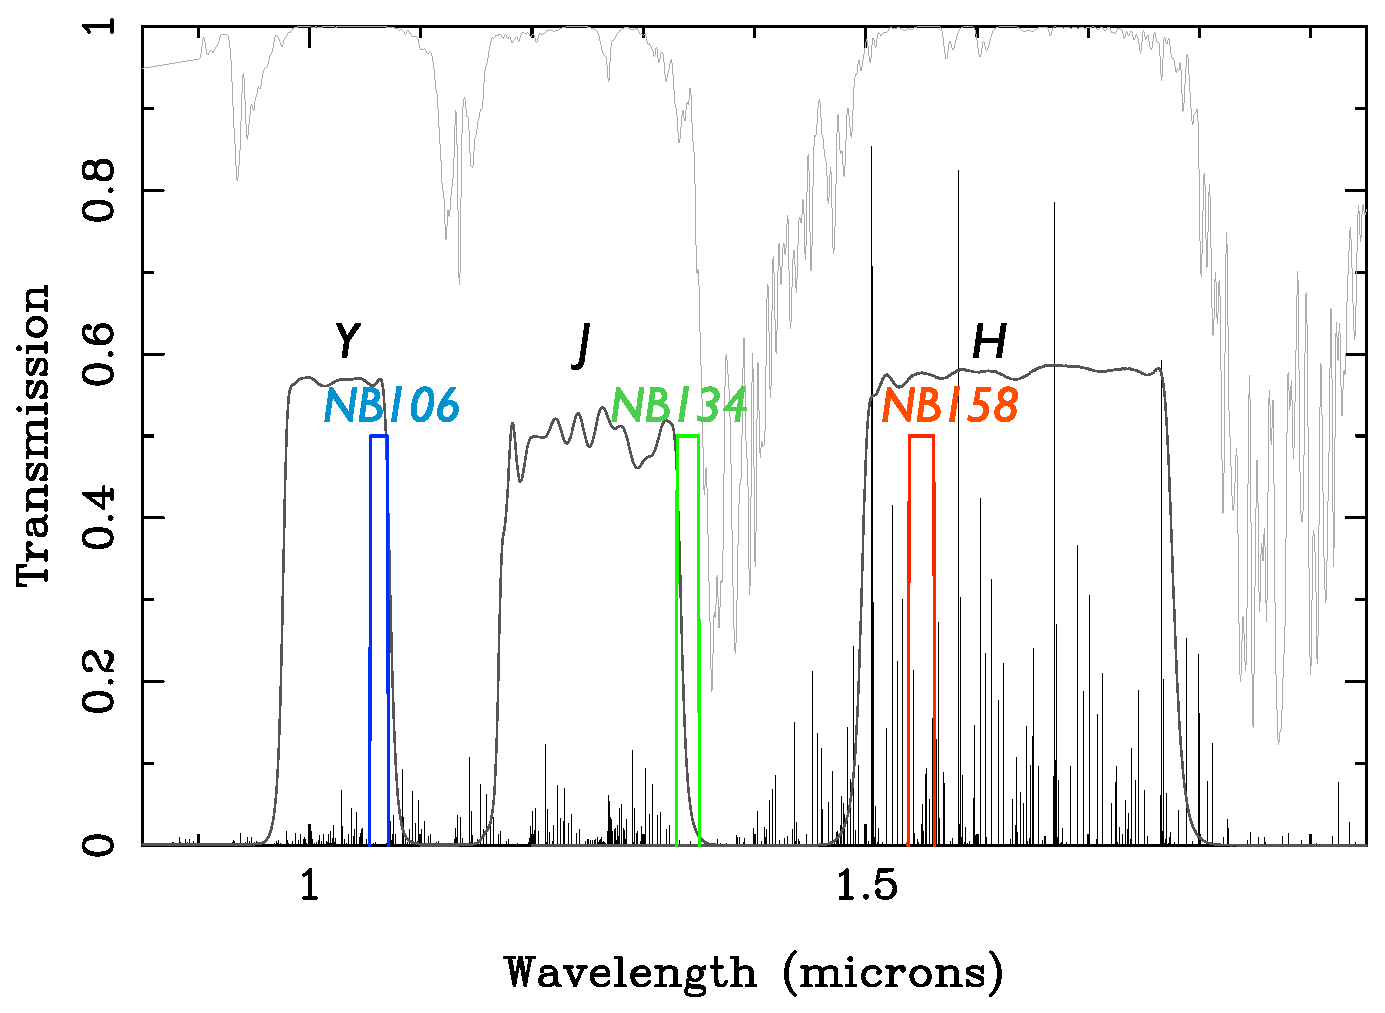
\includegraphics[width=80mm]{\thisdir figs/iwata_pg_filters_nbf01vd.eps}
}
\caption{
Transmission curves of NBFs considered. Transmission curves for $Y$,
 $J$, $H$-bands and the atomospheric transmission, and OH air glow
 strength (in arbitrary unit) are also shown.
}
\label{fig:iwata_filter_nbf}
\end{figure}



\par\noindent
[What should be clarified with ULTIMATE-SUBARU.]

\subsection{Proposed Observations}

\par\noindent
[Target objects: sample selection, number of objects, number of observing
fields, sky area.]

\par\noindent
[Observing modes: imaging or spectroscopy.]

\par\noindent
[Required observing time:]

\par\noindent
[Special requirements for ULTIMATE-SUBARU other than baseline
specifications, if any.]

\subsection{Synergy and Competitions}

\subsubsection{Synergy with TMT}

\subsubsection{Competitions with other facilities}

Instruments for 8--10m class telescopes.

ELT instruments.

Space-based projects.

\bibliographystyle{apj}
\bibliography{\thisdir nbf}
